\documentclass{scrartcl}
\usepackage[latin1]{inputenc}
\usepackage[T1]{fontenc}
\usepackage[ngerman]{babel}
\usepackage{amsmath}
\usepackage{amssymb}
\usepackage{icomma}
%\usepackage[dvips]{graphicx}
%\usepackage{floatflt}
%\usepackage{enumitem}
%\usepackage{babel}
\usepackage{blindtext}
%\usepackage{showframe}
\usepackage{wrapfig}
\def\BILD{\rule{0.4\textwidth}{4cm}}

\usepackage{graphicx}
\usepackage{placeins}
\usepackage{multirow}
\usepackage{subfig}
\usepackage{url}

\renewcommand{\topfraction}{.85}
\renewcommand{\bottomfraction}{.7}
\renewcommand{\textfraction}{.15}
\renewcommand{\floatpagefraction}{.66}
\renewcommand{\dbltopfraction}{.66}
\renewcommand{\dblfloatpagefraction}{.66}
\setcounter{topnumber}{9}
\setcounter{bottomnumber}{9}
\setcounter{totalnumber}{20}
\setcounter{dbltopnumber}{9}
\setlength{\intextsep}{0cm plus1cm minus1cm}
\pdfminorversion = 5
\usepackage{setspace}
\onehalfspacing

\begin{document}
\title{Versuch 6: Versuche zu den Abbe'schen Ideen der Bildentstehung
  beim Mikroskop}


\date{25.10.2010}


\author{Gruppe 5a: Gia-Danh Lam, Nils Haldenwang}

\maketitle
\tableofcontents

\section{Einleitung}

Unter Vernachl�ssigung von Linsenfehlern lassen sich mit der
geometrischen Optik \textit{ideale} Bilder konstruieren. Um aber die
tats�chliche Leistungsf�higkeit optischer Systeme zu untersuchen, muss
man die stets und unvermeidlich auftretende Beugung mit in Betracht
ziehen. Die erste Modellvorstellung eines durch Beugung entstehenden
Bildes entwickelte Ernst Abbe im Zusammenhang mit dem Mikroskop. Im
Folgenden werden die Abbe'schen Grundgedanken zur Bildentstehung unter
Frauenhofer Bedingungen und mit parallelem, koh�rentem Licht
durchgef�hrt. Die folgenden beiden Grundgedanken liegen der Abbe'schen
Theorie der Bildentstehung durch Beugung zu Grunde:

\begin{enumerate}
\item F�llt Licht auf ein Objekt, so entstehen unweigerlich
  Beugungseffekte. Durch Superposition der entstehenden
  Elementarwellen lassen sich Aussagen �ber den Wellenverlauf der
  Lichtstrahlen treffen. In Bild \ref{fig: Grundgedanke} ist der
  Gegenstand das Gitter G. Die roten, parallel zur optischen Achse
  verlaufenden Strahlen werden durch die Brechung der Linse genau in
  deren Brennpunkt $M_0$ geb�ndelt. Die gr�nen und blauen Strahlen
  sind durch die 1. und 2. Ordnung der Beugung entstanden. Sie treffen
  nicht parallel zur optischen Achse auf die Linse und werden demnach
  auch nicht im Brennpunkt $M_0$ fokussiert, sondern in den dazu
  verschobenen Brennpunkten $M_1$ und $M_2$. Alle parallelen
  Strahlenb�ndel, welche zu einem Beugungsmaximum n geh�ren, werden
  also in einem Brennpunkt $M_n$ in der Brennebene fokussiert. Alle
  $M_n$ stellen dabei die sog. \textit{Beugungsfigur} des Objektes
  dar.


\item Die Brennpunkte $M_n$ k�nnen als punktf�rmige Lichtquellen
  angesehen werden. Das Bild entsteht durch die Interferenz der
  von den Punkten $M_n$ ausgehenden Elementarwellen.
\end{enumerate}

\begin{figure}[htb!]
  \centering
  \mbox{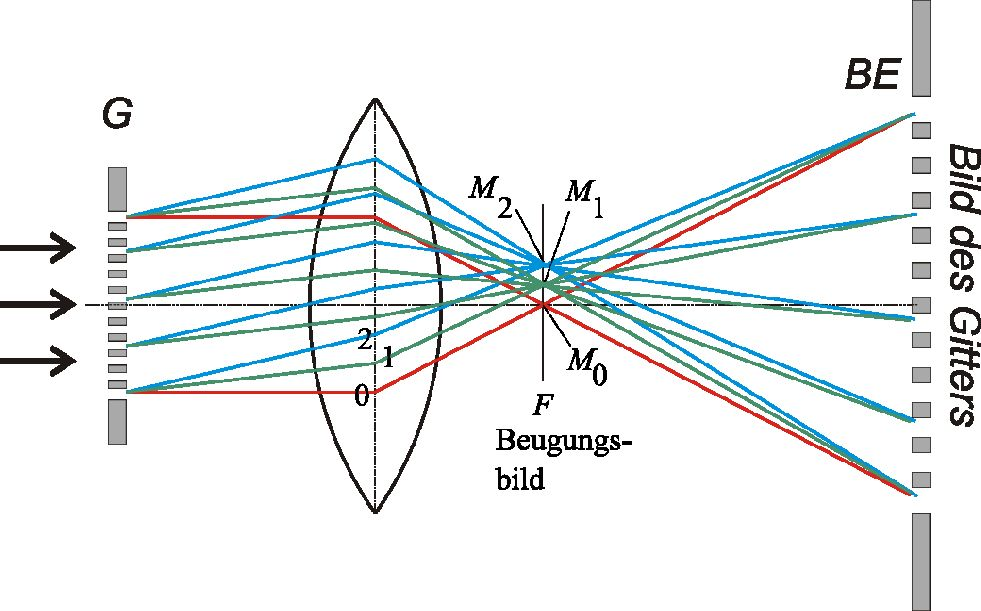
\includegraphics[width=75mm]{pics/2-000}}
  \caption{Darstellung der Bildentstehung nach Abbe}%
  \label{fig: Grundgedanke}%
\end{figure}



\section{Mikroskop aus zwei Linsen}

\section{Untersuchung der Diffraktionsplatte}
\subsection{Messung der Gitterkonstante}
\subsubsection{reales Bild}
\subsubsection{Beugungsbild}
\subsubsection{Ergebnis}

\subsection{Ver�nderungen am Beugungsmuster}
Im Folgenden soll das Bild  durch Manipulation des Beugungsmusters das
ver�ndert werden.  Zun�chst stellen wir die Spaltblende in die
Brennebene der Objektivlinse.  Den Spalt stellen wir erst einmal auf maximale
Gr��e um den Aufbau entsprechend zu justieren, sodass die
Beugungsfigur mittig auf dem Schirm zu sehen ist.  Nun blenden wir die
unerw�nschten Maxima durch Reduzieren der Spaltblende aus. Die
Projektionslinse verschieben wir nun wieder zur�ck, um das Bild auf
dem Schirm sehen zu k�nnen.  Im oberen Bildbereich ist das breite
Gitter zu sehen, im unteren das schmale Gitter.

\subsubsection{Verwendung der 0. Ordnung allein}
% TODO: Bilder einf�gen.

Das reale Bild zeigt einen gleichm��ig ausgeleuchteten Schirm.  Nach
Abbes verhalten sich die Beugungsmaxima wie Punktlichtquellen, aus
deren Interferenz das Bild erzeugt wird.  Da nur das 0. Maximum an der
Bilderzeugung beteiligt ist, kann keine Interferenz stattfinden,
sodass der Schirm aussieht, als werde er von einer einzelnen
Punktlichtquelle beleuchtet.

\subsubsection{Verwendung der 0. und 1. Ordnung des breiten Gitters}

Der obere Teil des Bildes zeigt die Struktur des breiten Gitters, da
nun auch die ersten Beugungsmaxima an der Bilderzeugung beteiligt
sind. Dem gegen�ber ist der untere Bereich relativ gleichm��ig
ausgeleuchtet, da f�r das schmale Gitter weiterhin nur das 0. Maximum
das Bild beeinflusst.

\subsubsection{0., 1., und 2. Ordnung der breiten Gitters}

Beide Gitter erscheinen in ihrem jeweiligen Bereich auf dem Schirm.
Dies ist exakt der nach den vorherigen Untersuchungen und der Theorie
von Abbes erwartete Effekt. Das Licht mindestens dreier Beugungsmaxima jeden
Gitters wird nun von der Blende hindurch gelassen, sodass diese
miteinander interferieren und ein Bild erzeugen k�nnen.

\subsubsection{Dreifachspaltblende}

Mittels einer V-f�rmigen Dreifachspaltblende an Stelle der
einfach Spaltblende wird nun das 1. Beugungsmaximum des breiten
Gitters ausgeblendet. Das 1. Maximum des schmalen Gitters wird jedoch
weiterhin hindurch gelassen.  Da nun lediglich die Bildinformationen
des schmalen Gitters verbleiben ist auch nur dieses zu sehen, und zwar auf dem gesamten
Schirm.

\subsection{Untersuchungen mit dem Kreuzgitter}

Die Diffraktionsplatte wird durch ein kreuzgitter ersetzt und die
Dreifach-Spaltblende durch einen einstellbaren, drehbaren Spalt.
Zun�chst wird die Spaltbreite auf ihren maximalen Wert eingestellt und
dann sukzessive verkleinert. Wir beobachten dabei das reale Bild des
Kreuzgitters und untersuchen danach das Beugungsmuster durch
entsprechende Verschiebung der Projektionslinse.

\subsubsection{Vertikale Stellung des Spalts}

Es ist zu beobachten, dass die  vertikalen Linien des Bildes immer
st�rker verblassen bis sie schlie�lich nicht mehr sichtbar sind und
man nur noch die waagerechten Linien erkennen kann. Die nicht
ausgeblendeten verbliebenen Maxima sind vertikal in einer Reihe
angeordnet. Es ist also kein Maximum der vertikalen Gitterlinien mehr
beteiligt, somit kann von ihnen auch kein Bild mehr auf dem Schirm
entstehen.

\subsubsection{Horizontale Stellung des Spalts}

In der horizontalen Spaltstellung bietet sich ein der vertikalen
Spaltstellung sehr �hnliches Bild, es ist lediglich um 90$^\circ$
gedreht. Dieses mal verblassen beim Verkleinern des Spalts die
waagerechten Linien, bis schlie�lich nur noch vertikale Linien zu
sehen sind. Ein Blick auf das Beugungsbild liefert eine waagerechte
Reihe von Maxima. Es hat kein Maximum der waagerechten Linien mehr
Einfluss auf das Bild, sodass diese folglich nicht mehr zu sehen sind.

\subsubsection{Diagonale Stellung des Spalts}

Wir drehen den Spalt nun in die Diagonale, also ca. um einen Winkel
von 45$^\circ$ nach links ( vom Laser aus gesehen ). Beim Verringern
der Spaltbreite verschwimmen nun sowohl waagerechte, als auch
vertikale Gitterlinien und es erscheinen diagonale Linien, welche um
90$^\circ$ zum Spalt gedreht sind. Das
Beugungsbild zeigt Beugungsmaxima in diagonaler Linie, die wie
bei den vorherigen Versuchen auch senkrecht zu den Linien im Bild steht. Dies ist
wenig verwunderlich, da gleiche Beugungsmuster nach Abbe auch gleiche
Bilder erzeugen. Der Abstand der Linien im Bild wird nun aber wohl ein
anderer sein, denn die Abst�nde der Maxima in der Diagonalen
unterscheiden sich von den vertikalen oder senkrechten um den Faktor $\sqrt{2}$.

\section{Fazit}

\end{document}
